\documentclass[a4paper,11pt]{article}

\usepackage{ucs}
\usepackage[utf8]{inputenc}
\usepackage{fontenc}
\usepackage{graphicx}
\usepackage{amsmath}
\usepackage{amssymb}
\usepackage{color}
\usepackage{algorithm}
\usepackage{algorithmic}
\usepackage{tikz,graphicx}
%\usepackage[dvips]{hyperref}

\date{01/01/14}

\newcommand{\myred}[1]
{\textcolor{red}{\bf {#1}}
}


\begin{document}
 \title{Pareto fronts for MiniZeno Benchmarks}

\maketitle

\section{Definition and notations}
\subsection{The Domain}
\ldots is that of MiniZeno \myred{to be completed}

\subsection{The Instances}
An instance is defined by
\begin{itemize}
 \item $n$ central cities, with costs/risks $c_1, \ldots, c_n$ plus the initial and goal cities. By abuse of notation, $c_i$ will mean the city itself as well as its cost/duration, the initial and goal cities will be denoted by $c_I$ and $c_G$ respectively.
 \item two arcs from each of the central cities to respectively the initial and final cities, with same flight durations $d_1, \ldots, d_n$;
 \item $p$ planes, initially in $c_I$;
 \item $t$ persons, initially in $c_I$, to be carried to $c_G$.
\end{itemize}

Without loss of generality, we can assume that the pairs $(d_i, c_i)$ are pairwise distinct (otherwise, the 2 cities can be ``merged'' and the resulting $n-1$ cities problem is equivalent to the original $n$ cities problem).

\subsection{The Constraints}
\begin{itemize}
 \item Symmetry, as already ensured by having the same duration $d_i$ from $c_G$ to $c_i$ than from $c_i$ to $c_G$ for all $i\in[1,n]$;
 \item Shortest path \myred{to be completed : si l'on considère une version simplifiée sans arcs entre les villes centrales, cette condition est trivialement vérifiée. À voir si la généralisation aux instances avec arcs ne pose pas de problème.}
\end{itemize}

\section{Pareto Front}
\noindent
{\bf Proposition}: possible Pareto-optimal plans and plans where each person visits only one central city.\\

{\bf Proof}: We consider a person visiting two central cities $c_{i_1}$ and $c_{i_2}$, resulting in a plan $P$, instead of only, $c_{i_1}$, resulting of the plan $P_1$, or only, $c_{i_2}$, resulting of the plan $P_2$. For an additive cost, it is clear that the cost of $P$ will be strictly higher that the cost of the plan $P_1$ or $P_2$. \myred{TODO : Cas où le second objectif est un risque. Cela pose problème car si le max des $c_i$ par lequel passe le plan $P$ n'est pas $c_{i_1}$ ou $c_{i_2}$, $P$, $P_1$ et $P_2$ ont le même risque. Il est également possible qu'ils aient le même makespan, auquel cas si $P_1$ ou $P_2$ appartient au front, alors $P$ également et on a un exemple où la proposition n'est plus vraie. D'un point de vu pratique cela dépend si l'on veut favoriser des plans plus courts ou non mais en ne considérant que les plans vérifiant la proposition on arriverait au même front}
If we consider the makespan, and thanks to the shortest path constraint, the path from $C_{i_1} \to C_G$ is shorter than $C_{i_1} \to \ldots \to C_{i_2} \to C_G$.\\ There is two possibilities :
\begin{itemize}
\item The makespan of the plane with the hightest makespan is modified (and thus higher). As it is also the makespan of the plan we can conclude that the makespan of this plan is higher.
\item The total makespan of the plan is not modified.
\end{itemize}

In both cases we can conclude that the plan where at least one person visits more than one city is Pareto-dominated by the plan where this person visits only one city.

\subsection{Pareto-optimal Plans}
A Possibly Pareto-optimal Plan (PPP) is thus defined by 
\begin{itemize}
 \item $t$ central cities, one for each person on her way to $c_G$ -- with indices $i_0, \ldots, i_{t-1}$
 \item $t-p$ central cities, with indices $i_{t}, \ldots, i_{2t-p-1}$ for the return flights of planes that have carried the persons to $c_G$ and fly back to $c_I$, assuming that all planes will end up in $c_G$ as any last return flights would be useless. 
 \item A schedule for the corresponding $4t-2p$ arcs. Note that there exists many feasible schedules, i.e., schedules that actually are feasible plans for $p$ planes.
\end{itemize}

\noindent
{\bf Cost/risk of a PPP}: Given $C = (c_{i_j})$, a $2t-p$-uple of cities, the cost (or the risk) of {\bf any} plan using (only) these cities are uniquely determined.
\[ 
Cost(C) = \sum_{j=0}^{2t-p-1} c_{i_j} \;\;\;;\;\;\; Risk(C) = Max\{c_{i_j} \;;\; j=0, \ldots, 2t-p-1\} 
\]

\noindent
{\bf Makespan of a PPP}: The makespan of the PPP is thus that of the shortest schedule that uses the $4t-4$ arcs in a feasible way. \\

\noindent
{\bf Bounds on the makespan of a PPP}: Trivial upper and lower bounds for the shortest makespan of a PPP $C$ are respectively $M_S(C)$, the makespan of the sequential plan (i.e., that of the plan for a single plane that would carry all persons one by one), and $M_L(C)$, the makespan of the perfect plan where none of the $p$ planes would ever stay idle.

\begin{eqnarray*}
 M_S(C) = 2 \sum_{j=0}^{2t-p-1} d_{i_j} \\
 M_L(C) = \frac{M_S(C)}{p}
\end{eqnarray*}

A much tighter upper bound can be rapidly obtained by greedily parallelizing the trips of the different places, see below.

\section{Counting PPPs}
\subsection{Cities}
The possible $2t-2$ visited cities  take values among the $n$ central cities.
There are hence at most $n^{(2t-p)}$ possible tuples. However, such set contains many redundancies, that can easily be removed by ordering the indices:

\noindent
{\bf Definition}: an {\it admissible} PPP-tuple is a vector of $2t-p$ cities $c_{i_j}, j=0, 2t-p-1 ; i_j\in[1,n]$ such that $i_j \geq i_{j+1}$ for all $j\in[0,t-1]$ (eastbound flights with passengers) and $i_j \geq i_{j+1}$ for all $j\in[t+1, 2t-p]$ (westbound/return flights with no passengers).\\

{\bf Number of admissible PPP-tuples}: We can uniquely separate a PPP-tuple $c$ into two sub-tuples that we denote $a\in{A}$ and $b\in{B}$. Let consider the space $\Gamma^{m}_{k}$ of $m$-tuples such that $\forall u \in \Gamma^{m}_{k} \;\; ||u||_1 = k$. The cardinality of $\Gamma$ is the number of combinaisons with repetitions of $k$ elements into a set of $m$, i.e. $\begin{pmatrix}
m+k-1\\
k
\end{pmatrix}$.\\

It exists a bijection between $A$ and $\Gamma^{n}_{t}$ and another between $\Gamma^{n}_{t-p}$ and $B$. Hence it exists a bijection between the {\it admissible} PPP-tuple set and the cartesian product of $\Gamma^{n}_{t}$ and $\Gamma^{n}_{t-p}$. We can conclude that the number of PPP-tuple is the cardinality of $\Gamma^{n}_{t} \times \Gamma^{n}_{t-p}$, i.e. $\begin{pmatrix}
n+t-1\\
t
\end{pmatrix}
\begin{pmatrix}
n+t-p-1\\
t-p
\end{pmatrix}$.\\

{\bf Example}: $t=3$,$n=3$,$p=2$. The number of admissible PPP is 30.\\

{\bf Remark}: $A\times B \subset \mathbb{R}^{2p-t}$ and $\Gamma^{n}_{t} \times \Gamma^{n}_{t-p} \subset \mathbb{R}^{2n}$. Thus, if $2t-p > 2n$ it is more convenient to store the PPP as 2 elements as $\Gamma$. \myred{Remarque : Je me demande cependant quelle forme est la plus simple à manipuler en pratique}

\subsection{Plans}
All PPP-tuple can be ordered by cost/risk, independently of the schedule/plan that will actually be the optimal one, i.e. the one with shortest makespan.

\noindent
{\bf A Greedy Upper-Bound}: given a admissible PPP-tuple $c_0, \ldots, c_{2t-1}$, the greedy upper bound for its makespan $M_G$ is given by Algorithm 1.\\
{\bf Hint}: Start with the longest flight durations $d_{i_0}, \ldots, d_{i_p}$ \myred{$d_{i_{t-1}}$ il me semble} in parallel. When a plane reaches $c_G$, pick up next return flight (i.e., the longest remaining one). When a plane reaches $c_I$, pick up next onward flight (longest remaining too), etc.\\

\myred{L'algorithme écrit par du principe que les $d_i$ sont décroissants mais il est simple de l'écrire de sorte à ne plus avoir cette contrainte.}

\begin{algorithm}
\caption{Calculate $M_G(C)$}
\begin{algorithmic}
%\REQUIRE $n \geq 0 \vee x \neq 0$
%\ENSURE $y = x^n$
\STATE $maxE \leftarrow 0$
\STATE $maxW \leftarrow t$
\STATE $M_i \leftarrow 0 \; \forall i=1,\ldots,p$
\STATE $S_i \leftarrow EAST \; \forall i=1,\ldots,p$
\COMMENT Indicates the direction for the next flight of the plane i.

\WHILE{$maxW \neq 2t-p$}
\STATE $k \leftarrow \underset{i}{argmin}(M_i)$ \COMMENT First plane waiting (ie. arriving at $C_I$ or $C_G$)
\IF{$S_k = EAST$}
\STATE $M_k \leftarrow M_k + 2d_{c_{maxE}}$
\STATE $S_k \leftarrow WEST$
\STATE $maxE \leftarrow maxE + 1 $;
\ELSE
\STATE $M_k \leftarrow M_k + 2d_{c_{maxW}}$
\STATE $S_k \leftarrow EST$
\STATE $maxW \leftarrow maxW + 1 $;
\ENDIF
\ENDWHILE
\\
\WHILE{$maxE \neq t$}
\STATE $k \leftarrow \underset{i, S_i=EAST}{argmin}(M_i)$
\STATE $M_k \leftarrow M_k + 2d_{c_{maxE}}$
\STATE $S_k \leftarrow WEST$
\STATE $maxE \leftarrow maxE + 1 $;
\ENDWHILE
\\
\RETURN $\underset{i}{max}(M_i)$
\end{algorithmic}
\end{algorithm}

A PPP-tuples can then be pruned if its lower bound for makespan is worse than the greedy upper bound for makespan of another PPP-tuple whose cost is better.\\

\noindent
{\bf Greedy domination}: Given two admissible PPP-tuples $C$ and $C'$, $C$ {\it greedily dominates} $C'$ if $M_G(C) \leq M_L(C')$ and $Cost(C) \leq Cost(C')$\\

\myred{hopefully :-)} several PPP-tuples can be pruned that way.

\subsection{Computing the Shortest Makespan}
\myred{TODO: write a smart algorithm :-) Pas vraiment de meilleure idée pour le moment que de l'énumération avec backtrack (on peut l'appeler Branch and Bound) qui utilise les meilleures bornes de makespan de tous les PPP-tuples qui ont un meilleur coût ???}

\myred{RQ: Je propose une autre méthode sans backtrack. La preuve d'optimalité me semble un peu bancale ou incomplète mais j'obtiens la solution optimale même si les X exemples que j'ai essayé. En bonus, il permet de retrouver un plan optimal assez -facilement- au besoin ,même si à programmer cela semble une autre paire de manche. L'algorithme glouton est un cas particulier de la méthode.}

\subsubsection{Flight patterns}

It exists 3 different patterns that can be carried out by planes, represented by figure \ref{M1}, \ref{M2}, \ref{M3}. We can notice that the last one has to be performed by two planes and is non-preemptive (ie. once the first plane drops off the person at the central city, the other plane can pick her up later). These patterns result from the fact that if a plane is empty it should only fly to the west and to the east otherwise.\\

\begin{figure}
\centering
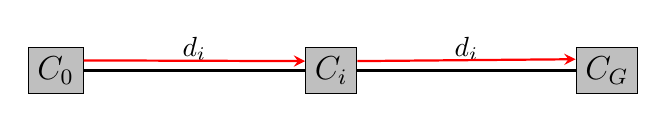
\begin{tikzpicture}
	% Villes
 \node[draw, fill=black!25] (0) at (-3.5,0) {\large $C_0$};
 \node[draw, fill=black!25] (2) at (0,0) {\large $C_i$};
 \node[draw, fill=black!25] (4) at (3.5,0) {\large $C_G$};

	% Liaison inter villes
 \draw[thick] (0)--(2) node[midway, above]{$d_{i}$};
 \draw[thick] (2)--(4) node[midway, above ]{$d_{i}$};

 \draw[thick,->,>=stealth, red] (0.20) -- (2.160);
 \draw[thick,->,>=stealth, red] (2.20) -- (4.160);
 
\end{tikzpicture}
\caption{\label{M1} Pattern 1}
\end{figure}
%,->,>=stealth

\begin{figure}
\centering
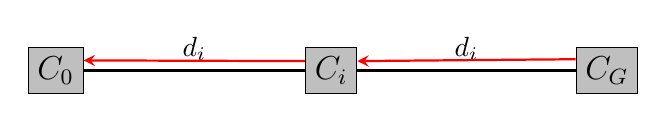
\begin{tikzpicture}
	% Villes
 \node[draw, fill=black!25] (0) at (-3.5,0) {\large $C_0$};
 \node[draw, fill=black!25] (2) at (0,0) {\large $C_i$};
 \node[draw, fill=black!25] (4) at (3.5,0) {\large $C_G$};

	% Liaison inter villes
 \draw[thick] (0)--(2) node[midway, above]{$d_{i}$};
 \draw[thick] (2)--(4) node[midway, above]{$d_{i}$};

 \draw[thick,<-,>=stealth, red] (0.20) -- (2.160);
 \draw[thick,<-,>=stealth, red] (2.20) -- (4.160);
 
\end{tikzpicture}
\caption{\label{M2} Pattern 2}
\end{figure}
%,->,>=stealth

\begin{figure}
\centering
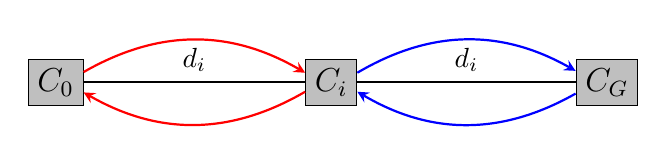
\begin{tikzpicture}
	% Villes
 \node[draw, fill=black!25] (0) at (-3.5,0) {\large $C_0$};
 \node[draw, fill=black!25] (2) at (0,0) {\large $C_i$};
 \node[draw, fill=black!25] (4) at (3.5,0) {\large $C_G$};

	% Liaison inter villes
 \draw[thick] (0)--(2) node[midway, above]{$d_{i}$};
 \draw[thick] (2)--(4) node[midway, above]{$d_{i}$};

 \draw[thick,->,>=stealth, red] (0.20) to[bend left] (2.160);
 \draw[thick,<-,>=stealth, red] (0.-20) to[bend right] (2.200);

  \draw[thick,->,>=stealth, blue] (2.380) to[bend left] (4.160);
 \draw[thick,<-,>=stealth, blue] (2.340) to[bend right] (4.200);
 
\end{tikzpicture}
\caption{\label{M3} Pattern 3}
\end{figure}
%,->,>=stealth

\noindent
Thus, the last pattern is the only one that implies -interactions- beetween planes.\\

\noindent
We can also notice that, for a given city $i$, the time per plane to complete a pattern in the same for each pattern.\\

\noindent
We will denote the cardinal of the first and the second pattern in a PPP by, respectively, $\alpha_E$ and $\alpha_W$ and for last pattern by $\beta$. We will refer to the eastern part and the western part of $\beta$ by, respectively, $\beta_E$ and $\beta_W$.\\

\subsubsection{Repartition of patterns for an admissible PPP}

For a given PPP, $\beta$ can be bounded as follows : $0 \leq \beta \leq t-p$.
As a Pattern 3 requires a move from $c_I$ to the east and another one from $c_G$ to the west, a tighter bound is obtained by the number of components of $W$ that can be associated to the elements of $E$.\\

{\bf Example}: $$C = (3,1,1)(2,1)$$
The first bound equals to 2 but if we take a closer look, it is impossible to perform a Pattern 3 with the city 2 since it is not present in the tuple $E$.\\

\noindent
Given $\beta$, the number of each pattern is fully qualified : 
$$
\left\{
\begin{matrix}
\beta \\
\alpha_W = t-p-\beta \\
\alpha_E = t - \beta \\
\end{matrix}\right.$$

\noindent
{\bf Proposition}: The Greedy Upper-Bound is optimal for an admissible PPP and $\beta = 0$.\\

\noindent
\myred{TODO: Preuve ? Cela me semble assez évident.}\\

\subsubsection{The algorithm}

The main idea is to compute the shortest makespan for each value of $\beta$, given an admissible PPC, and to take the minimum value.\\

\noindent
Notice that it is possible for a given $\beta$ to have multiple choices for the cities involved in Pattern 3. However, we can reduce the choice to only one by $\beta$ as explained below \myred{(TODO : le prouver :D)}.\\

\noindent
For a given $\beta$, we compute a greedy value for the duration requiered for each person to be transported to $C_G$. We first start with $\beta$ pattern, without taking into account the number of planes involved. We always chose first the city $i$ that implies the longest flight.

{\bf Example}: 

$t=5$, $p=3$, $d=(2,4,6)$\\ $C = (3,2,2,1,1)(2,1) \implies 0 \leq \beta \leq 2$. 

We chose $\beta = 1$ with the pattern 3 to be executed around the city 1.

\begin{center}
\begin{tabular}{|c||c|c|l|}
    \hline
    & Pattern & Cities & Time \tabularnewline
    \hline \hline
    $t_1$ & $\beta$ & $c_1 || c_1$ & $T_1=4$  \tabularnewline 
    \hline \hline
    $t_2$ & $\alpha_E$ & $c_3$ & $T_2=12$  \tabularnewline 
    \hline
    $t_3$ & $\alpha_E$ & $c_2$ & $T_3=8$  \tabularnewline
    \hline
    $t_4$ & $\alpha_E$ & $c_1$ & $T_4=4$  \tabularnewline
    \hline \hline
    $t_5$ & $\alpha_W + \alpha_E$ & $c_1+c_1$ & $T_5=8$  \tabularnewline
    \hline
 \end{tabular}
\end{center}

We can now compute the makespan of the optimal plan according to the durations we obtained for each passenger.\\
\begin{enumerate}
\item For each $t_i, \forall i\in\{\beta+1,\ldots, p+1\}$, $M(p_j) \leftarrow M(p_j) + T_i$ with $j = \underset{1 \leq k \leq p}{argmin}(M(p_k))$.
\item For each $t_i, \forall i\in\{p+1,\ldots, t\}$, $M(p_j) \leftarrow M(p_j) + T_i$ with $j = \underset{1 \leq k \leq p}{argmin}(M(p_k))$. \myred{RQ : l'étape 2 peut ne pas exister en fonction de $C$ et de $\beta$}
\item For each $t_i, \forall i\in\{1,\ldots, \beta\}$, $M(p_{j_1}) \leftarrow M(p_{j_1}) + T_i$ and $M(p_{j_2}) \leftarrow M(p_{j_2}) + T_i$, with $p_{j_1}$ and $p_{j_2}$ the two planes with the best current makespan.
\end{enumerate}

\noindent
{\bf Example}: \\

\noindent
With the previous table.\\

\begin{tabular}{c l }
    $p_1:$ & $T_2+T_1=16$ \tabularnewline
    $p_2:$ & $T_3+T_5=16$ \tabularnewline
    $p_3:$ & $T_4+T_1=12$ \tabularnewline
\end{tabular}

~\\ Thus, the minimal makespan is 16. We also found that $M_S(C)=16$, then this is the optimal makespan.\\

\noindent
{\bf Proposition}: We can always construct a valid plan with the makespan returned by the algorithm.

\myred{TODO : Donner la méthode de construction. Est-ce assez comme preuve ?}\\

\noindent
{\bf Proposition}: The makespan returned by the algorithm is optimal for the PPP C and the cities involved in the pattern 3.\\

{\bf Proof}: 
\begin{itemize}
\item The incompressible time needed to carry out all passengers, according to a repartition of patterns (and cities involved in pattern 3) is $T = 2\sum_{i\in\{1,\ldots, \beta\}} T_i + \sum_{i\in\{\beta + 1,\ldots, p\}}T_i$. A theoretical optimal plan with this pattern repartition is a plan without any waiting point for any plane.
\item The above algorithm gives the optimal partition of the set of times $\{T_i\}_i\}$ into $p$ (with the constraint that $T_i$ with $i=\in\{1,\ldots, \beta\}$ is present into 2 different subsets). Then, if a plan can be constructed with such a makespan, it is optimal for the PPP and the repartition of patterns.
\item As it exists a method to construct such a plan, we can conclude that the algorithm is optimal for the PPP C and the cities involved in the pattern 3. We can also conclude that, in this case, it is always possible to construct a plan without any waiting point.
\end{itemize}

\noindent
{\bf Number of iterations for an admissible PPP C}: In the worst case, we have $0 \leq \beta \leq t-p$, for each value of $\beta$ we have then $\begin{pmatrix} t-p \\ \beta \end{pmatrix}$ possibilities. Thus, still in the worst case, we will perform $\sum_{i=0}^{t-p}\begin{pmatrix} t-p \\ i \end{pmatrix} = 2^{t-p}$ iterations.

\myred{RQ : Ca fait beaucoup en théorie... Peut être qu'on peut choisir les villes du pattern 3 de manière intelligente. Après, sur des petites instances cela reste faisable vu le coût de l'itération (ie le problème à 3 villes, 3 personnes et 2 avions donne 48 itérations pour l'ensemble des PPC - hors PPC que l'on peut pénaliser au cours du calcul -)}

\subsubsection{The cities involved in pattern 3 ?}

The sum of time spent by all planes is $T = 2\sum_{i\in\{1,\ldots, \beta\}} T_i + \sum_{i\in\{\beta + 1,\ldots, p\}}T_i$.\\


\noindent
We denote by $S_{\beta}(C)$ the set of cities that can be involved in a pattern 3, for a given PPP $C$ and a given value of $\beta$.\\


\noindent
It is clear that if $\beta = 1$ and $S_1(C)$ reduced to 2 distinct elements $c_k$ and $c_l$ such that $d_k < d_l$, then we obtain 2 distinct sums $T$ and $T'$. The difference gives $T' - T = 2d_l - 2d_k + d_k - d_l = d_l - d_k > 0$


\myred{RQ : Bon, je vois pas encore trop comment prouver qu'il faut choisir la ville dont les arcs adjacents sont minimaux (ça m'a l'air vrai et je n'arrive pas à trouver de contre exemple). Si c'était effectivement le cas, on peut généraliser aux à $S_1(C)$ de cardinal quelconque, puis, je pense, à n'importe quel $\beta$. Le fait de fixer $\beta$ fixerait alors également la ou les villes à choisir de manière unique : prendre les villes de $S_1(C)$ dont les arcs sont de poids minimal.}

\section{Obtaining the Pareto Front}
\begin{itemize}
 \item For all admissible PPP-tuples, compute the cost/risk, the lower bound and the greedy upper bound on the makespan. 
 \item Remove the greedily-dominated ones
 \item For the remaining ones, compute the plan with shortest makespan
\end{itemize}

\myred{RQ: Il me semble que le mieux est de prendre l'ensemble des PPP admissibles qui ont le même second objectif (par valeur croissante) et d'essayer pour une valeur $\beta$ donnée cet ensemble de PPP plutôt que de tester toutes les valeurs de $\beta$ pour un PPP donné. On commence par $\beta = 0$ ce qui revient exactement à l'algorithme glouton donné plus haut. On peut ainsi éliminer progressivement des PPP comme on l'aurait fait juste avec l'algorithme glouton.}

\end{document}
